\documentclass[a4paper]{article}

\usepackage[english]{babel}
\usepackage[utf8]{inputenc}
\usepackage{graphicx}
\usepackage{epsfig}
\usepackage{amsmath}
\usepackage{graphicx}

%\usepackage{natbib} \setlength{\bibsep}{4.0pt}
\usepackage[colorinlistoftodos]{todonotes}
\usepackage{a4}
%\usepackage{cite}
%\usepackage{amssymb}
\usepackage{color}
\usepackage{lineno}
\usepackage{ulem}
\usepackage{enumerate}
\usepackage{comment}

\usepackage[left=2.5cm,right=2cm,top=2.5cm,bottom=2.cm]{geometry} 

%% for long url reference
\usepackage{hyperref}
\usepackage{url}
\makeatletter
\def\url@mystyle{%
  \@ifundefined{selectfont}{\def\UrlFont{\sf}}{\def\UrlFont{\small\ttfamily}}}
\makeatother
\urlstyle{my}



\renewcommand{\thefootnote}{\alph{footnote}}
\renewcommand{\topfraction}{.99}
\renewcommand{\bottomfraction}{.99}

\title{Drift velocity and Electric Field measurement with LArIAT Run I and Run II data}

%%%%%%%%%%%%%%%%%%%%%%%%%%%%%%%%%
\begin{document}
%%%%%%%%%%%%%%%%%%%%%%%%%%%%%%%%%
\def\Journal#1#2#3#4{{#1} {\bf #2}, #3 (#4)}
\def\etal{{\it et\ al.}}
\def\numunue{\nu_\mu\rightarrow\nu_e}
\def\numunutau{\nu_\mu\rightarrow\nu_\tau}
\def\nuebar{\bar\nu_e}
\def\nue{\nu_e}
\def\nutau{\nu_\tau}
\def\numubar{\bar\nu_\mu}
\def\numu{\nu_\mu}
\def\ra{\rightarrow}
\def\numubarnuebar{\bar\nu_\mu\rightarrow\bar\nu_e}
\def\nuebarnumubar{\bar\nu_e\rightarrow\bar\nu_\mu}
\def\osc{\rightsquigarrow}
\def\inteni{{\cal I}_{pot}}
\def\fmerit{{\cal F}}
%%%%%%%%%%%%%%%%%%%%%%%%%%%%%%%%%
\begin{flushright}
{\tt version 1.0}\\ 
\today
\end{flushright}
\vspace*{0.6cm}
%%%%%%%%%%%%%%%%%%%%%%%%%%%%%%%%%
\linenumbers
%%%%%%%%%%%%%%%%%%%%%%%%%%%%%%%%%
\begin{center}
{\Large \bf Drift velocity and Electric Field measurement with LArIAT Run I and Run II data} 
\vspace*{1.6cm}
\setcounter{footnote}{0}  
\def\A{\kern+.6ex\lower.42ex\hbox{$\scriptstyle \iota$}\kern-1.20ex a}
\def\E{\kern+.5ex\lower.42ex\hbox{$\scriptstyle \iota$}\kern-1.10ex e}
\small
\newcommand{\Aname}[2]{#1}
\def\titlefoot#1{\vspace{-0.3cm}\begin{center}{\bf #1}\end{center}}

Authors: Jonathan Asaadi, Flavio Cavanna, Bonnie Fleming, Will Foreman, Elena Gramellini,  Greg Pulliam , Jen Raaf, Andrzej M. Szelc,   Jason St. John\\

\end{center}
\vspace*{1cm}

\noindent Please send comments to: elena.gramellini@yale.edu


%%%%%%%%%%%%%%%%%%%%%%%%%%%%%%%%%
%% ABSTRACT
%%%%%%%%%%%%%%%%%%%%%%%%%%%%%%%%%
%\newpage
\begin{abstract}
In this note, we describe several methods to determine the electric field, drift velocity and drift time in the LArIAT TPC main drift volume. 
A precise measure of these quantities is fundamental to properly leverage on the basic capabilities of a LArTPC: tracking and calorimetry. In fact, the position of hits in the drift direction and electron life time are directly affected by the values of the electric field, drift velocity and drift time.\\

We find for the 90.3 K temperature of the argon in the center of the cryostat an electric field value of 486.5 V/cm using the single line drawing with a drift velocity of 1.51 mm/$\mu s$ and a drift time of 311.3 $\mu s$. Results consistent with these values are found as well using cathode to anode piercing tracks.

\end{abstract} 

%%%%%%%%%%%%%%%%%%%%%%%%%%%%%%%%%
%% Table of content
%%%%%%%%%%%%%%%%%%%%%%%%%%%%%%%%%
\tableofcontents


%%%%%%%%%%%%%%%%%%%%%%%%%%%%%%%%%
%% SECTION 1: Introduction
%%%%%%%%%%%%%%%%%%%%%%%%%%%%%%%%%
\newpage
\section{Introduction}\label{sec:Introduction} \label{sec:Intro}
%%%%%%%%%%%%%%%%%%%%%%%%%%%%%%%%%%%%%%%%%%%%%%%%%%%%%%%%%%%%%%
The electron drift time (and by extension the drift velocity) is a fundamental parameter to the working principal of a LArTPC. By knowing the speed of the electron drift we are able to project the position of the charge back into the TPC volume, enabling 3D reconstruction. The drift velocity is determined by the electric field in the drift volume, so having a good handle on the electric field is essential. In this note we present two methods to calculate the electric using the measured detector properties such as temperature, pressure, voltage and current of the LArIAT TPC during its operation in Run-I and II. (A very similar calculation can be done for Run-III using slightly modified voltages.)

We first define some of the basic working parameters of the LArIAT experiment in Section \ref{sec:Def} and then move on showing two methods of calculating the electric field strength expected in the drift volume. In Section \ref{sec:elDiagram} we use the simplified single-line diagram of the electric circuit along with the values recorded in ACNET to calculate the voltage on the cathode. Using this voltage we then calculate the electric field strength, drift velocity, and drift time. In Section \ref{sec:CAMethod} we use an alternative method, identifying cathode-to-anode piercing tracks (tracks which cross the cathode and wire planes as they traverse the TPC) to extract the drift time. From this drift time the drift velocity is calculated, and then the electric field strength. 

These two methods yield results consistent with one another, giving us confidence that we understand the strength of the electric field present in the drift volume.

%%%%%%%%%%%%%%%%%%%%%%%%%%%%%%%%%%%%%%%%%%%%%%%%%%%%%%%%%%%%%%%%%%%%%%%%%%%%%%%%%
\subsection{Definitions: electric field, drift velocity and drift time }\label{sec:Def}
%%%%%%%%%%%%%%%%%%%%%%%%%%%%%%%%%%%%%%%%%%%%%%%%%%%%%%%%%%%%%%%%%%%%%%%%%%%%%%%%%
As shown in Figure \ref{fig:driftregions}, the LArIAT TPC has three drift volumes, each of which has its own electric field value. The main drift volume is defined as the region between the cathode plane and the shield plane (C-S). Note that the shield plane wires are uninstrumented. This is the region for which the majority of this note will be focused on for calculating the electric field, drift velocity, and drift times.

The other two drift regions are those between the shield plane and the induction plane (S-I), and between the induction plane and the collection plane (I-C). The electric field in these regions is chosen to satisfy the charge transparency condition to allow for 100$\%$ transmission of the drifting electrons through the shield and then the induction planes.

\begin{figure}[htb]
\centering
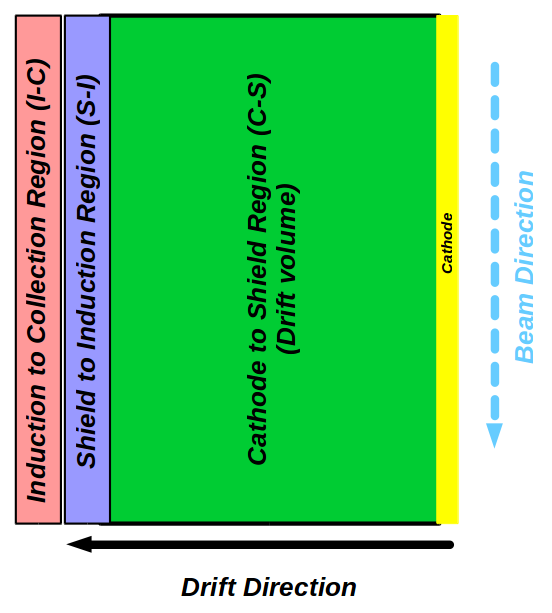
\includegraphics[scale=0.35]{./images/DriftRegions.png}\\
\caption{Schematic of the three drift regions inside the LArIAT TPC. The main drift volume between the cathode and the shield plane (C-S), the region between the shield plane and the induction plane (S-I), and the region between the induction plane and the collection plane (I-C).}
\label{fig:driftregions}
\end{figure}

Table \ref{tab:voltages} provides the voltages applied to the shield, induction, and collection plane for Run-I, and Run-II. These voltages were changed in Run-III to maintain the transparency condition when the wire spacing was changed. For data taken in Run-I and Run-II the spacing between the S-I and I-C regions was a constant 4~mm.

\begin{table}[htpb]
\centering
\caption{Anode planes voltages}
\label{tab:voltages}
\begin{tabular}{lll}
\hline
\multicolumn{1}{|l|}{VShield} & \multicolumn{1}{l|}{VInduction} & \multicolumn{1}{l|}{VCollection} \\ \hline
\multicolumn{1}{|l|}{-298.75} & \multicolumn{1}{l|}{-18.5}      & \multicolumn{1}{l|}{338.5}       \\ \hline
                              &                                 &                                 
\end{tabular}
\end{table}

Once we have the electric field strength we can calculate the drift velocity ($v_{drift}$) using the relationship
\begin{equation} v_{drift} = \mu(E_{field},T) E_{field}, \label{eq:vd}
\end{equation}
where $\mu$ is the electron mobility, which depends on the electric field and on the temperature (T). The empirical formula for this dependency is described in ~\cite{WWW} and shown in Figure \ref{fig:EV} for several argon temperatures.

\begin{figure}[htb]
\centering
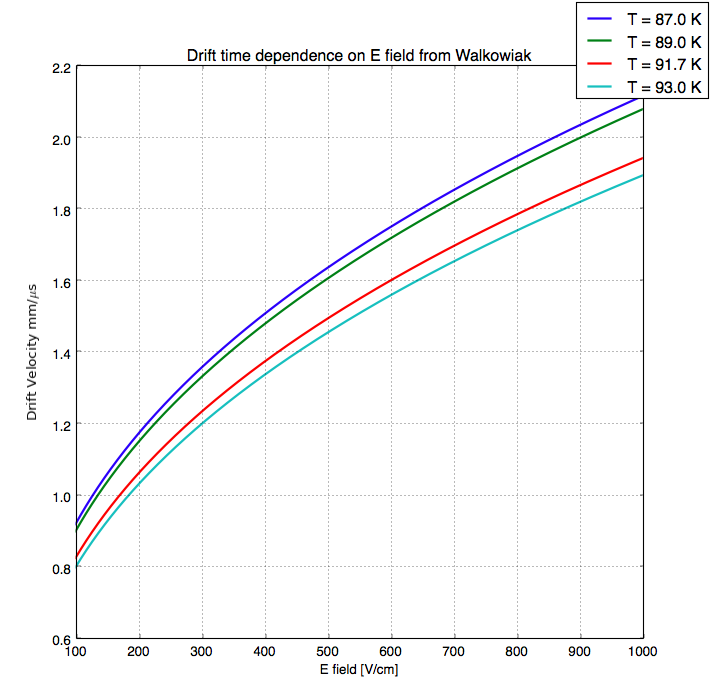
\includegraphics[scale=0.45]{./images/Walkowiak.png}\\
\caption{Drift velocity dependence on electric field for several temperatures. The slope of the line at any one point represents the electron mobility for that given temperature and electric field.}
\label{fig:EV}
\end{figure}

In order to determine the temperature inside the TPC we measure the pressure in the cryostat gas volume and calculate the pressure at the center of the TPC. From this pressure and the boiling point curve of argon, we calculate the temperature. The pressure at the surface of the liquid argon is maintained by the cryosystem at $\sim$20~psi as shown in Figure \ref{fig:pressure} for a period of 13 days with an average pressure of 20.0 $\pm$.0.4 psi.

\begin{figure}[htb]
\centering
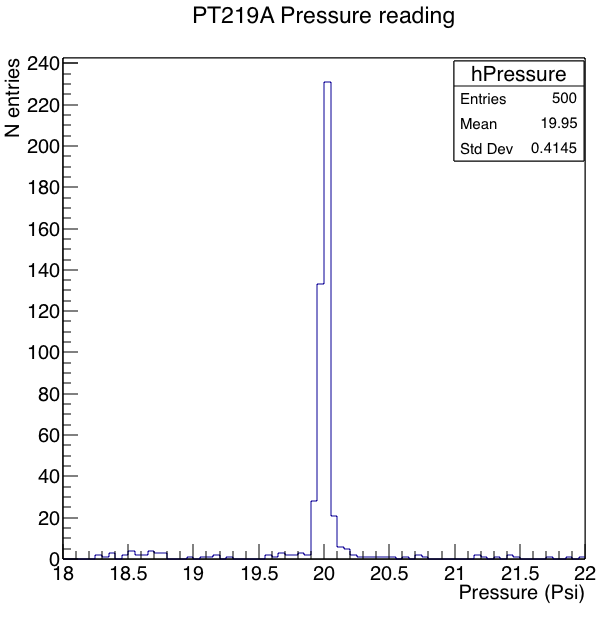
\includegraphics[scale=0.45]{./images/Pressure.png}\\
\caption{PT219A pressure distributions for 13 days (2017/6/23 - 2017/7/5).}
\label{fig:pressure}
\end{figure}

In order to calculate the pressure (and subsequently the temperature) in the middle of the TPC, we consider about 40 cm of argon from the ulage surface to the center of the TPC. This volume of argon raises the pressure 0.79 psi to give a pressure at the center of the TPC of 20.79 psi. According to the NIST tables, [\textcolor{red}{reference}], this corresponds to a temperature of 90.7 K. This is the temperature value we will utilize throughout this note.

It is worth noting that LArIAT is equipped with three temperature probes inside the liquid argon volume. One probe at the bottom (TE213A in Figure \ref{fig:cryo}), one in the middle (TE314A in Figure \ref{fig:cryo}) and one on the top of the cryostat (TE212A in Figure \ref{fig:cryo}). These probes give a similar temperature reading to the one we just calculate, as listed in Table \ref{tab:temp}, but since these probes were never calibrated to an absolute number, we instead rely on the pressure measurement presented above.

\begin{table}[h!]
\centering
\caption{Average temperatures measured at the top, middle and bottom in the LArIAT cryostat.}
\label{tab:temp}
\begin{tabular}{|c|c|c|}
\hline
Top Probe Temp (TE212A) & Middle Probe Temp (TE214A)   & Bottom Probe Temp (TE213A)  \\ \hline
91.7 $\pm$ 0.7 K &  91.8 $\pm$ 0.7 K                   & 93.3 $\pm$ 2.7 K       \\ \hline
\end{tabular}
\end{table}

\begin{figure}[htb]
\centering
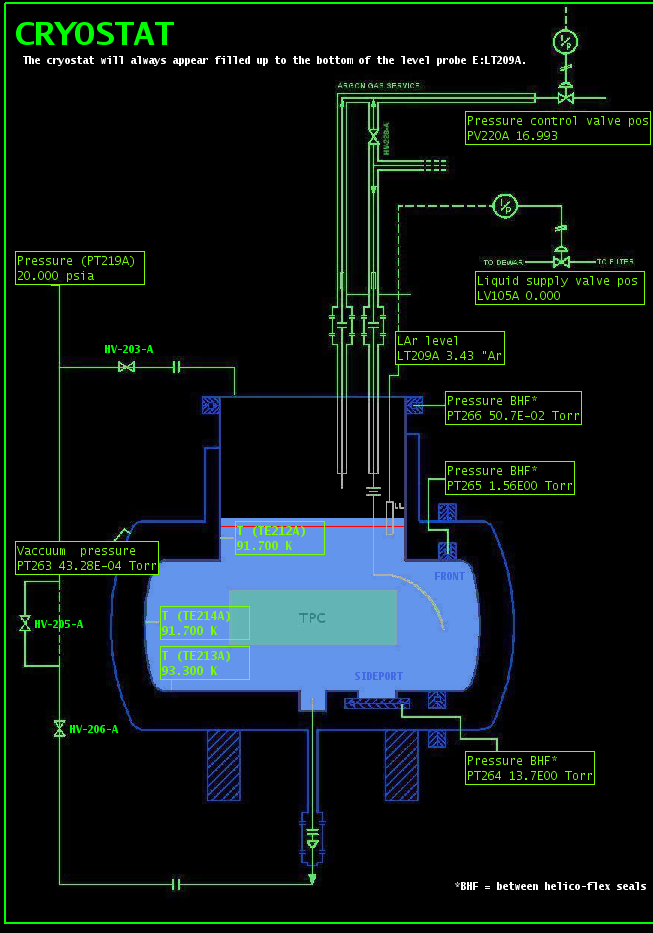
\includegraphics[scale=0.45]{./images/cryopic.png}\\
\caption{Scheme of LArIAT cryostat and cryo probes.}
\label{fig:cryo}
\end{figure}

Once the drift velocity is determined, the relationship between the drift time ($t_{drift}$) and the drift velocity is trivially given by
\begin{equation}
t_{drift} = \Delta x/v_{drift}, \label{eq:drifttime}
\end{equation}
where $\Delta x$ is the distance between the two regions (for the regions of the wire planes, this is 4~mm).

Table \ref{tab:Efields} reports the values of the electric field, drift velocity, and drift times for the smaller drift volumes. The next few paragraphs describe how these quantities are calculated.

 
\begin{table}[]
\centering
\caption{Electric field and drift velocities in LArIAT smaller drift volumes}
\label{tab:Efields}
\begin{tabular}{|l|l|l|}
\hline
& Shield-Induction & Induction-Collection \\ \hline
E$_{filed}$ &                 700.625 V/cm        &                892.5  V/cm             \\ \hline
v$_{drift}$ &                   1.73  mm/$\mu$s   &                  1.90 mm/$\mu$s        \\ \hline
t$_{drift}$ &                   2.31  $\mu$s      &                   2.11 $\mu$s          \\ \hline

\end{tabular}
\end{table}

With these basic parameters established, we can now move on to calculating the electric field in the main drift region (between the cathode and the shield plane).

\newpage
\clearpage
\newpage
%%%%%%%%%%%%%%%%%%%%%%%%%%%%%%%%%%%%%%%%%%%%%%%%%%%%%%%%%%%%%%%%%%
\section{E field using electrical diagram}\label{sec:elDiagram}
%%%%%%%%%%%%%%%%%%%%%%%%%%%%%%%%%%%%%%%%%%%%%%%%%%%%%%%%%%%%%%%%%%
The electric field strength in the LArIAT main drift volume can be determined knowing the voltage applied to the cathode, the voltage applied at the shield plane, and the distance between them. We assume the distance between the cathode and the shield plane to be 470 mm and any length contraction due to the liquid argon is negligibly small ($\sim 2$mm).

The voltage applied to the cathode can be calculated using Ohm's law and the circuit diagram shown in Figure \ref{fig:circuit}. The voltage supplied by the Glassman power supply during Run-I and Run-II was 23.5~kV. Between the Glassman power supply and the cathode was a set of two of filter pots for emergency power dissipation, one at each end of the feeder cable, each with an internal resistance of 40~M$\Omega$. 

Thus all that is needed to determine the electric field strength is the output current of the Glassman. However, an error in the values as recorded by Fermilab's Accelerator Controls Network (ACNET) was found during this investigation. As shown in Figure \ref{fig:currentMeasurement}, ACNET records an average current of 0.04172 mA from the power supply ($\sim$40$\mu$A).  This is now known to be unreliable, due to an uncalibrated scale factor. 

However, this number is inconsistent with the know resistance inside the TPC. The LArIAT TPC has four 1~G$\Omega$ resistors in parallel (250 M$\Omega$ equivalent) serving as the voltage divider across each of the 24 steps of the field cage. This means that the equivalent resistance across the whole TPC should be ~6~G$\Omega$. Thus the expected current out of the Glassman should be 
\begin{equation}
I_{expected} = \frac{V_{power supply}}{R_{Total}} = \frac{23.5 kV}{6.08 G\Omega} = 3.8 \mu A \approx 4 \mu A
\end{equation}

After further investigation it was concluded that the recording of the values in ACNET were likely mis-calibrated by a factor of 10 and thus the correct current to assume from the Glassman should be corrected to 0.00417 mA = 4$\mu$A.

\begin{figure}[hp]
\centering
\begin{minipage}{0.45\textwidth}
\centering
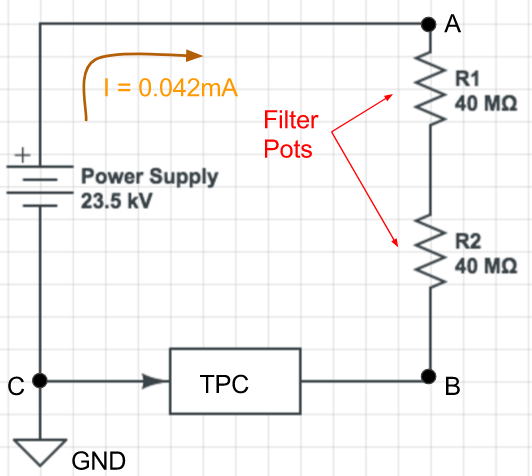
\includegraphics[width=3in]{images/CircuitLArIAT.png}
\caption{LArIAT HV simple schematics.}
\label{fig:circuit}
\end{minipage}\hfill
\begin{minipage}{0.45\textwidth}
\centering
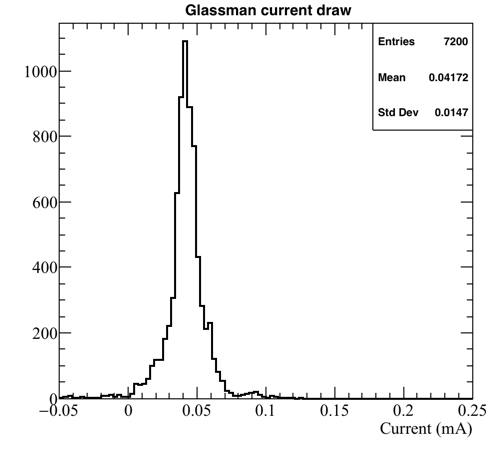
\includegraphics[width=3in]{images/glassman_current_20160525-30.png}
\caption{Current reading from the Glassman between May 25th and May 30th 2016 (typical Run2 conditions).}
\label{fig:currentMeasurement}
\end{minipage}
\end{figure}

Thus, using this corrected current, the voltage at the cathode is calculated as:

\begin{equation} V_{BC}=V_{PS} - I_{corrected}*R_{eq} = -23.5kV + 0.00417mA*80M\Omega = -23.17 kV, \label{eq:VBC}
\end{equation}
where I is the current and R$_{eq}$ is the equivalent resistor representing the two filter pots. The electric field, drift voltage and drift time are then calculated to be

\begin{equation}E_{filed} = \frac{V_{BC} - V_{shield}}{\Delta x} = 486.54 \textit{ V/cm}
\end{equation}
\begin{equation}v_{drift} = \mu E_{field} = 1.5097 \textit{ mm/$\mu$s}
\end{equation}
\begin{equation}t_{drift} = \frac{\Delta x}{v_{drift}} = 311.316 \textit{ $\mu$s.}
\end{equation}



\newpage
\section{E field using cathode-anode piercing tracks}\label{sec:CAMethod}
\begin{figure}[b]
\centering
\begin{minipage}{0.45\textwidth}
\centering
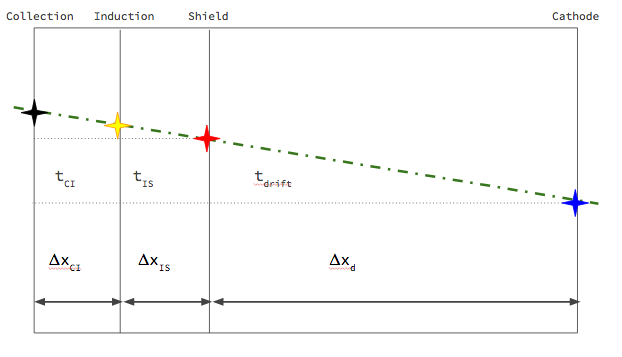
\includegraphics[width=3in]{images/TPCCrossSectionView.png}
\caption{Pictorial representation of the YX view of the TPC. The distance within the anode planes and between the shield plane and the cathode is purposely out of proportion to illustrate the time difference between hits on collection and induciton. A ACP track is shown as an example.}
\label{fig:Scheme}
\end{minipage}\hfill
\begin{minipage}{0.45\textwidth}
\centering
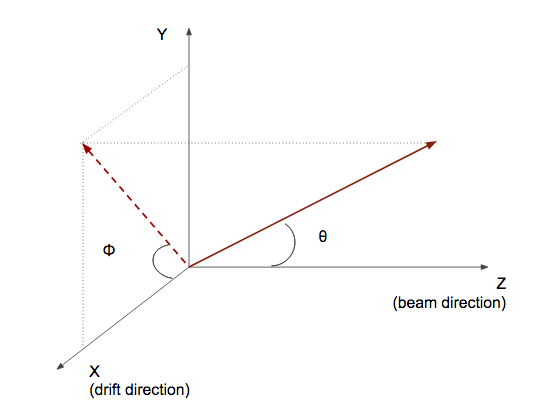
\includegraphics[width=3in]{images/AngleDef.png}
\caption{Angle definition in the context of LArIAT coordinates system.}
\label{fig:AngleDef}
\end{minipage}
\end{figure}

In this section, we propose a method to measure the drift time (and consequently drift velocity and electric field) using TPC data.
The basic idea is simple:
\begin{itemize}
\item[0.] select events with only 1 reconstruced track 
\item[1.] select tracks that cross both anode and cathode,
\item[2.] identify the first and last hit of the track,
\item[3.] measure the time difference between these two hits ($\Delta t$),
\item[4.] derive the drift time from this time difference.
\end{itemize}
We use cosmic data (see section \ref{sec:SampleSelectionCA}) and work under the following assumptions: 
\begin{itemize}
\item [A1.] the selected tracks are muons in the MIP region
\item [A2.] the time it takes for a muon to cross the chamber ($\sim$ns) is irrelevant compared to the charge drift time ($\sim$ hundreds of $\mu$s).
\end{itemize}

We select events with only one recontructed track to assure the track considered in the analysis is associated with the trigger.
We select anode-cahode piercing tracks (ACP tracks in what follows) because their hits span the full drift lenght of the TPC, see figure \ref{fig:Scheme}. It is important to define where the first and last hit of the tracks are located. The definition of the last hit is easy: it is the hit closest to the cathode. The definition of the first hit is a bit more complicated. A track that crosses the anode planes will deposit charge in the small drift volumes (CI and IS). We calculated the dift time in IS and CI in table \ref{tab:Efields}: $\Delta t_{IS} = 2.31  \mu s$  and $\Delta t_{CI} = 2.11 \mu s $ respectvely. This is to say that the position of the first hit  matters when calculating the drift time at the microsecond precision.
Single hits on the collection plan will not form a 3D object. This means that we can safely exclude that the reconstruction of ACP tracks starts at the cathode plane (black point in figure \ref{fig:Scheme}). Understanding if the first hit of a track in on the induction or on the shield plan is more complicated. For now, we'll take an uncertainty hit of 2.3 $\mu$s.


One of the main features of this method is that it doesn't rely on the measurement of the trigger time. Since $\Delta t$ is the time difference between the first and last hit of a track and we assume the charge started drifting at the same time for both hits (assumption A2), the measurement of the absolute beginning of drift time $t_0$ is unnecessary. 


\subsection{Andode-Cathode Piercing Tracks Sample Selection}\label{sec:SampleSelectionCA}

The data samples used for this measurement span RunI and RunII. The data are divided into three independent subsamples: RunI positive polarity data, RunII positive polarity data and RunII negative polarity data. Since we're interested in cosmics, this organization is arbirtary and only dictated by the subsamples availability.
More details are shown in table \ref{tab:samples}, while the samweb definitions are defined at the end of \href{https://redmine.fnal.gov/redmine/projects/lardbt/wiki/Recommended_SAM_Datasets}{this wiki page}.

\begin{center}
\begin{table}[htb]
  \begin{center}
    %\resizebox{0.45\textwidth}{!}{%
    \begin{tabular}{c|c|c|c}
      \multicolumn{4}{c}{\textbf{Summary of Samples}} \\
      \hline \hline
       Run Period & LArIATsoft Version & Data Polarity  & SamWeb definition\\
       \hline
       Run-I & \verb!v06_34_01! & Positive &  \verb!Lovely1_Pos_RunI_elenag_v04!\\
       \hline
       Run-II & \verb!v06_34_01! & Positive  & \verb!Lovely1_Pos_RunII_elenag_v04! \\
       \hline
       Run-II & \verb!v06_34_01! & Negative  & \verb!Lovely1_Neg_RunII_elenag_v04! \\
       \hline
       \end{tabular}%}
    \caption{Summary of the data samples used for the Anode-Cathode Piercing tracks study. }
    \label{tab:samples}
    \end{center}
\end{table}
\end{center}

For each sample, the same event selection is used: we outline it in what follows.
\begin{itemize}
\item \textbf{Time Stamp Filter}

A filter is used to select events which occured outside the beam window. This is because the beam is mainly focused in the Z direction, so ACP tracks are unlikely to occur during the beam spill. Cosmics events typically occur 5.5 seconds past the beam spill, and therefore the events are filtered using the following LArIATsoft settings

\begin{verbatim}
tfilt:      @local::lariat_timestampfilter

# ====================================================================
# Specify range of events to select.  For Run I/II:
#   - pedestal events:  ~ 0.  - 1.2 sec
#   - beam events:      ~ 1.2 - 5.5 sec
#   - cosmic events:    ~ > 5.5 sec
#   (default selects ALL events)
physics.filters.tfilt.T1:                       5.5
physics.filters.tfilt.T2:                       100.
physics.filters.tfilt.RequireRawDigits:         true

\end{verbatim}


\item \textbf{LArTPC Reconstruction}

Events are then reconstructed inside the TPC. Since we only want ACP tracks, we select tracks that satisfy the following requirements

\begin{itemize}
\item vertical position (Y) of first and last hits within $\pm$ 18 cm from TPC center (avoid Top-Bottom tracks) 
\item horizonatl position (Z) of first and last hits within 2 and 86 cm from TPC front face (avoid throughoing tracks) 
\item longest track with track lenght greater than 48 cm
\item angle from the drift direction (phi in figure \ref{fig:AngleDef}) smaller than 50 deg 
\item angle from the beam direction (theta in figure \ref{fig:AngleDef}) grater than 60 deg
\end{itemize}




\end{itemize}

Tracks passing all these selection requirements are used for the $\Delta t$ calculation.


\subsection{Hit timing information}\label{sec:HitTime}
For each track passing our selection, we loop through the associated hits in order to retrieve the timing information. Hits on the collection and hits on the induction are treated separately. Three types of timing information are provided per each hit: tStart, tPeak and tEnd. The quantities tStart and tEnd are used to identify a region of interest on the signal wave form in each wire. This ROI is represent the time boundary where a fit for the signal peak is performed. The variable tPeak stores the fitted value for the time of the hit. For this analysis, we use \verb!gaushitfinder! and the variable tPeak as a measure of the hit time.


Figure \ref{fig:RunIPosACP} represents the difference in time between the last and first hit of the selected ACP tracks for RunI Positive Polarity sample. The red histogram represents $\Delta$t calculated with hits on induction plan, while the blue histogram histogram represents $\Delta$t calculated with hits on the collection plan.
Figure \ref{fig:RunIIPosACP} and \ref{fig:RunIINegACP} are analougus to figure \ref{fig:RunIPosACP} for RunII Positive and Negative polarity respectively.

\begin{figure}[b]
\centering
\begin{minipage}{0.45\textwidth}
\centering
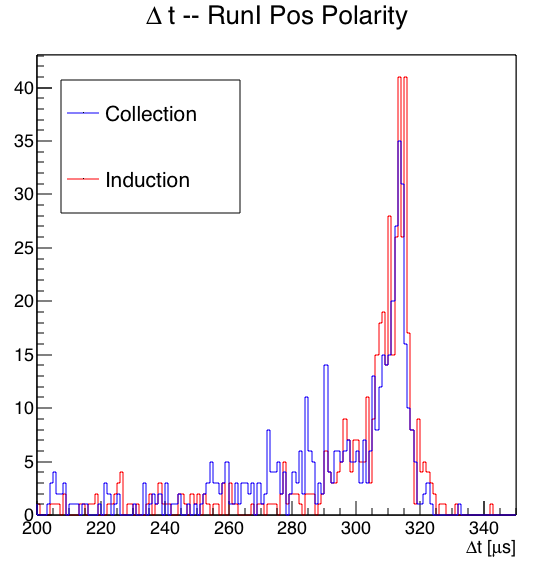
\includegraphics[width=3in]{images/ACPRunIPos.png}
\caption{$\Delta$t for Run I positive polarity data ACP selected tracks. The blue line represents hits on the collection plan, red induction.}
\label{fig:RunIPosACP}
\end{minipage}\hfill
\begin{minipage}{0.45\textwidth}
\centering
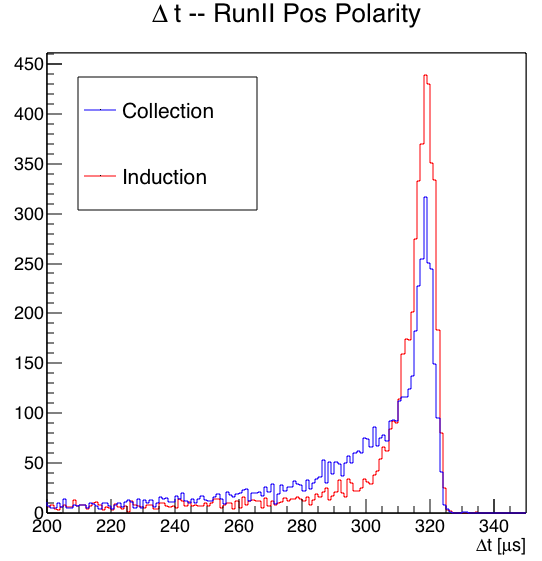
\includegraphics[width=3in]{images/ACPRunIIPos.png}
\caption{$\Delta$t for Run II positive polarity data ACP selected tracks.  The blue line represents hits on the collection plan, red induction.}
\label{fig:RunIIPosACP}
\end{minipage}\hfill
\begin{minipage}{0.45\textwidth}
\centering
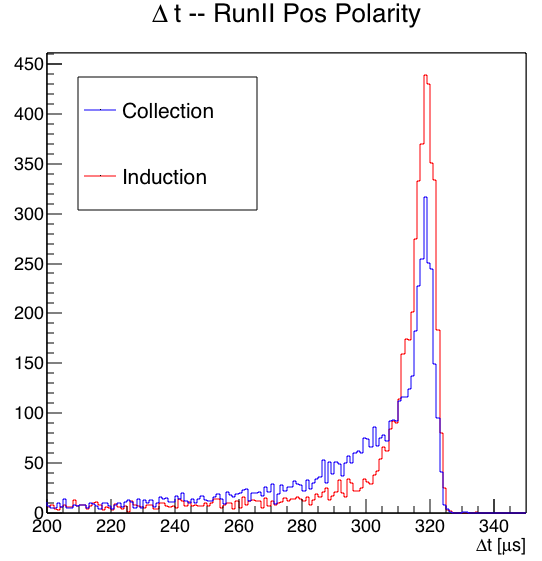
\includegraphics[width=3in]{images/ACPRunIIPos.png}
\caption{$\Delta$t for Run II negative polarity data ACP selected tracks.  The blue line represents hits on the collection plan, red induction.}
\label{fig:RunIINegACP}
\end{minipage}
\end{figure}

We fit with a gaussian the peak in figures  \ref{fig:RunIPosACP}, \ref{fig:RunIIPosACP} and \ref{fig:RunIINegACP}. An example of the fit is shown in figures \ref{fig:CollFit} and \ref{fig:IndFit}. We use the mean as our estimate of $\Delta t$ and the sigma as it error. The $\Delta t$ value for each distribution is shown in table \ref{tab:deltaTACP}.
\begin{figure}[b]
\centering
\begin{minipage}{0.45\textwidth}
\centering
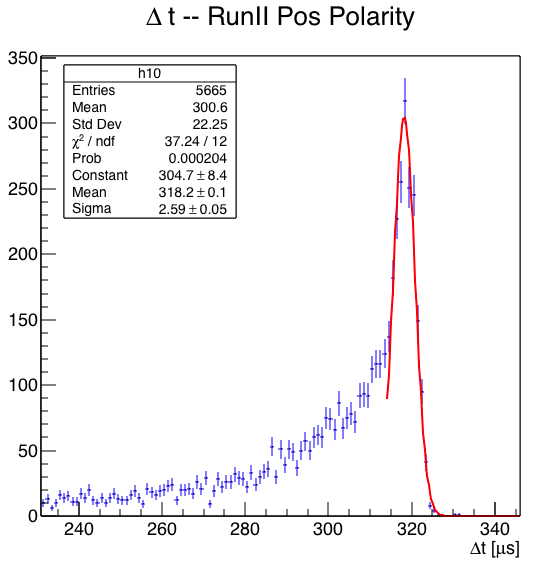
\includegraphics[width=3in]{images/CollectionFitRunIIPos.png}
\caption{Collection plan $\Delta$t fit  for Run I positive polarity data ACP selected tracks. }
\label{fig:CollFit}
\end{minipage}\hfill
\begin{minipage}{0.45\textwidth}
\centering
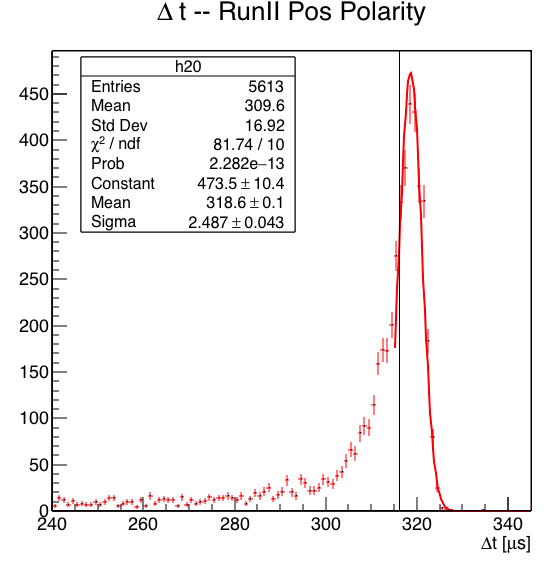
\includegraphics[width=3in]{images/InductionFitRunIIPos.png}
\caption{Collection plan $\Delta$t fit  for Run I positive polarity data ACP selected tracks. }
\label{fig:IndFit}
\end{minipage}
\end{figure}

\begin{center}
\begin{table}[htb]
  \begin{center}
    %\resizebox{0.45\textwidth}{!}{%
    \begin{tabular}{|c|c|}
      \multicolumn{2}{c}{\textbf{Delta t for ACP tracks}} \\
      \hline \hline
       Data Period  & $\Delta t$ [$\mu s$] \\
       \hline
       RunI Positive Polarity Induction & 313.7 $\pm$ 2.1 \\
       \hline
       RunI Positive Polarity Collection & 313.2 $\pm$ 2.6 \\
       \hline
       RunII Positive Polarity Induction &  318.6 $\pm$ 2.5\\
       \hline
       RunII Positive Polarity Collection & 318.2 $\pm$ 2.6 \\
       \hline
       RunII Negative Polarity Induction &  $\pm$ \\
       \hline
       RunII Negative Polarity Collection & $\pm$ \\
       \hline
       \end{tabular}
    \caption{$\Delta t$ for the different data samples used for the Anode-Cathode Piercing tracks study. }
    \label{tab:deltaTACP}
    \end{center}
\end{table}
\end{center}


For the RunII Positive polarity data, we scan plot the position of the peak as a function of the angle theta and phi. Figures \ref{fig:RunIPosACPTheta} and \ref{fig:RunIIPosACPPhi} show the trends.
\begin{figure}[b]
\centering
\begin{minipage}{0.45\textwidth}
\centering
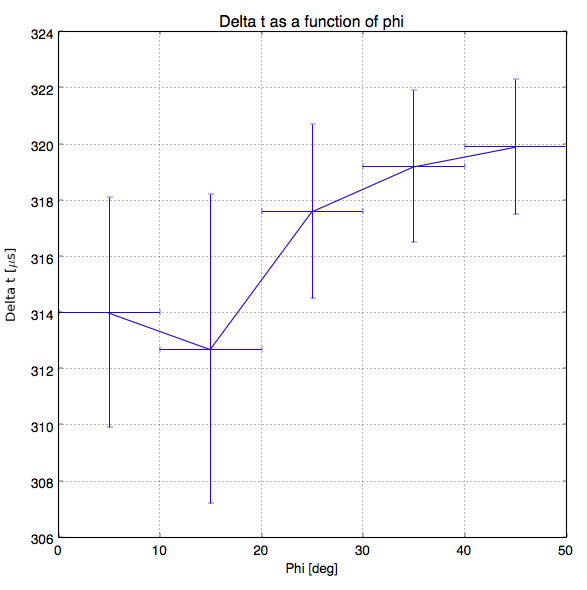
\includegraphics[width=3in]{images/CollectionFitRunIIPosPhi.png}
\caption{$\Delta$t for Run II positive polarity data ACP selected tracks as a function of Phi. }
\label{fig:RunIPosACPTheta}
\end{minipage}\hfill
\begin{minipage}{0.45\textwidth}
\centering
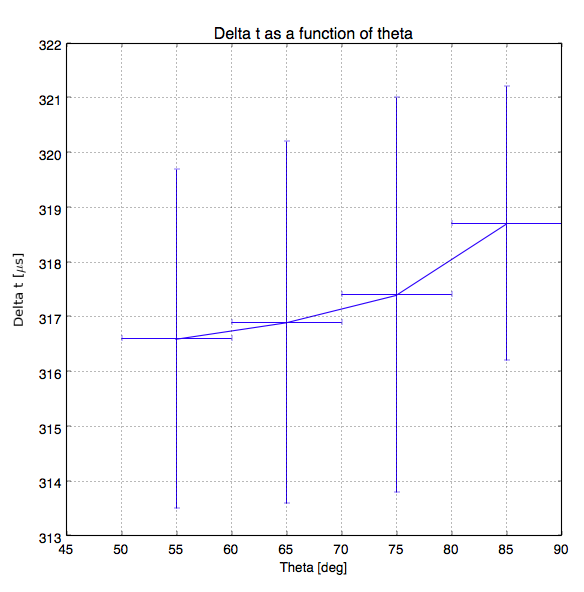
\includegraphics[width=3in]{images/CollectionFitRunIIPosTheta.png}
\caption{$\Delta$t for Run II positive polarity data ACP selected tracks as a function of Theta.}
\label{fig:RunIIPosACPPhi}
\end{minipage}
\end{figure}
\clearpage
\newpage

\newpage
%%%%%%%%%%%%%%%%%%%%%%%%%%%%%%%%%%%%%%%%%%%%%%%%%%%
\section{Results}\label{sec:Results}
%%%%%%%%%%%%%%%%%%%%%%%%%%%%%%%%%%%%%%%%%%%%%%%%%%%
The following table summarizes the results from the two methods described above.
\begin{center}
\begin{table}[htb]
  \begin{center}
    \begin{tabular}{c|c|c|c}
      \multicolumn{4}{c}{\textbf{Summary of Results}} \\
      \hline \hline
       Method & Drift Time [$\mu$s] & Drift velocity [mm/$\mu$s]  & Electric field [V/cm]\\
       \hline
       Electric circuit        & 311.3  & 1.51 & 486.5 \\
       \hline
       Crossing Tracks: Run I  &  & \\
       \hline
       Crossing Tracks: Run II &  & \\
       \hline
       \hline
       \end{tabular}%}
    \caption{Summary of the results. }
    \label{tab:ResultsFinal}
    \end{center}
\end{table}
\end{center}



\newpage
\clearpage
\appendix
%\section{Appendix 1: Crossing Muons} \label{appendix:CrossingMuon}
Particles with energies higher than $\approx$ 150 MeV can cross the TPC volume and exit the TPC without experiencing an interaction. We define as “crossing” each particle that exits the TPC fiducial boundaries.\\
These particles will then contribute only in filling the $N_{incident}$ histogram for each point of their track, meaning that for the energies related to the track points they are more likely to survive than to interact with Ar nuclei.\\

The percentage of crossing tracks from the Closed Box data sample are reported in Tab.\ref{tabellaCrossing}. In Fig.\ref{CrossingOBKinEn} the Incident and Final kinetic energy of crossing tracks in the Open Box sample is reported.
\begin{table}[ht!]
\centering
\begin{tabular}{|c|c|}
\hline
\textbf{Event Sample} & \textbf{Number of Events} \\ 
\hline \hline
Run I Negative Polarity Data Sample                                                                          & 486753           \\
\hline
After all selection cuts                                                                      & 2404             \\
\hline
Crossing tracks                                                                               & 858              \\
\hline
\% Crossing tracks over events that pass all cuts & 35.7 \%\\          
\hline
\end{tabular}
\caption{Crossing tracks after all the selection cuts for a subsample of Run-I data.} 
\label{tabellaCrossing}
\end{table}

\begin{figure}[h!]
\centering
\includegraphics[scale=0.45]{./images/OBparticles_crossingKinEn.png}
\caption{Initial and Final kinetic energy spectra for Crossing tracks ifor a subsample of Run-I data.}
\label{CrossingOBKinEn}
\end{figure}

We know the particles from the beamline which can exit the TPC boundaries will be mainly pions and muons. It is then natural to evaluate the percentage of contamination by muons in our "crossing particles" data sample. Since crossing muon tracks will be taken into account when filling the $N_{incident}$ histogram for the Pion cross section evaluation. The {\textbf{crossing muon contamination}} in $N_{incident}$ will then affect our measurement.

We agreed to provide an estimate for the contribution of "crossing muon" events via Monte Carlo simulation. We will then apply this "crossing muon contamination" correction on the $N_{incident}$ histogram made from the data sample.\\
We made a study of crossing track events from the MC sample of pions and muons (the incoming particles energy spectrum was re-weighted based on the beam profile). In Tab.\ref{tab:CrossingMC} we show the percentages of crossing pions and muons after our selection cuts, in case a fixed number of pions and muons are shot in our MC simulation. Muons are not strongly affected by our selection cuts and we see they're mostly crossing events (almost 76\% of the selected muon events are crossing tracks). Pion statistic is a bit more affected by our cuts than the muon's: 70.1\% of the pions that enter the TPC made it to pass all our selection cuts and only 32\% of them are crossing tracks, since most of them interact into the TPC volume.\\
% Considering crossing events, from Tab.\ref{tab:CrossingMC} we see:
% $$ \Big(\frac{\mu}{\pi}\Big)_{cross,cuts}^{MC, unweighted} \simeq 3 $$
% this is in case of same number of pions and muons shot via MC.
For our analysis, it is important to consider the relative fraction of pions and muons in the beam to get a proper estimate of the real crossing muon contamination of our sample. The muon to pion fraction from the beam composition is, for negative polarity runs (See Tab.\ref{tab:beamcomp1}): 
$$ \Big(\frac{\mu}{\pi}\Big)_{beam} \simeq 0.045 $$
%commented stuff - weird results - to be updated soon
Therefore if we weight by the beam composition the crossing muons to crossing pions ratio obtained before, we can get an average estimate over all energies for the $(\frac{\mu}{\pi})_{cross}$ we can expected in the Data:
$$ \Big(\frac{\mu}{\pi}\Big)_{cross,cuts}^{MC, weighted} \simeq  0.136 $$
The average MC estimate of the composition of Crossing Tracks sample is then: 88\% pions, 12\% muons.\\ 
% (on average - MC estimate): 
% Pi: 88 %
% Mu: 12 %
% (considering the beam composition and assuming ONLY Pi and Mu cross the TPC)

A more complete analysis has been made considering the crossing muon contamination in each energy bin of $N_{incident}$ histogram, as shown in Fig.\ref{CrossingMCNinc}, Fig.\ref{CrossingOBMuon} and Fig.\ref{CrossingFraction}. \\
The fraction of crossing muons in each energy bin of $N_{incident}$ histogram will actually make our denominator for cross section calculation higher then if we had only pions.
From the plot in Fig.\ref{CrossingFraction} we see the fractional contribution of crossing muons is quite flat, at least in the 50-650 MeV region.
We have decided to consider a uniform crossing muon contamination factor of the order of 10\% and to apply this correction in each energy bin of the $N_{incident}$ histogram made from our Data sample. This results in a 9\% reduction of the content of each energy bin. We will also assume a 20\% uncertainty on our estimate of the crossing muon contamination factor in $N_{incident}$, that will reflect in a $\approx$ 3\% systematic on the cross section measurement for each energy bin.

$$ N_{incident}^{data} \longrightarrow N_{incident}^{data, \mu corr} \text{ applied 9\% crossing $\mu$ contamination correction}$$
$$\sigma \approx \frac{N_{incident}^{data}}{N_{incident}^{data, \mu corr}} \text{ , } \Big(\frac{\Delta\sigma}{\sigma}\Big)_{sys}^{\mu corr} \simeq 3 \% $$ 


\begin{table}[ht!]
\centering
\begin{tabular}{|l|l|l|}
\hline
\textbf{Event Sample}                                                                                 & {\textbf{Pions}} & {\textbf{Muons}} \\ \hline \hline
MC sample                                                                                     & 118800 & 79200 \\ \hline
MC sample - particles that enter the TPC                                                      & 80603 & 76328 \\ \hline
After all selection cuts                                                                      & 56462 & 63146 \\ \hline
Crossing tracks                                                                               & 26035  & 58261 \\ \hline
\% Crossing tracks  & 32.3 \% & 76.3 \% \\ \hline
\end{tabular}
\caption{Crossing tracks after all the selection cuts for pions and muons (from MC).}
\label{tab:CrossingMC}
\end{table}


% \begin{figure}[h!]
% \begin{minipage}{0.5\textwidth}
% \includegraphics[width=\textwidth]{PionCrossingKinEn.png}
% \end{minipage}
% \begin{minipage}{0.5\textwidth}
% \includegraphics[width=\textwidth]{CrossMuKinEn.png}
% \end{minipage}
% \caption{Initial and Final kinetic energy spectra for Crossing Pion and Muon tracks from MC Sample.}
% \label{CrossingMCPionKinEn}
% \end{figure}

% \begin{figure}[h!]
% \centering
% \includegraphics[scale=0.4]{CrossMuPiKinEn.png}
% \caption{Initial kinetic energy spectra for Crossing Pion and Muon tracks from MC Sample weighted by beam composition.}
% \end{figure}

\begin{figure}[h!]
\begin{minipage}{0.5\textwidth}
\includegraphics[width=\textwidth]{./images/CrossingPiMu.png}
\end{minipage}
\begin{minipage}{0.5\textwidth}
\includegraphics[width=\textwidth]{./images/CrossingCBandMuMC.png}
\end{minipage}
\caption{$N_{incident}$ histogram for Crossing Pion and Muon tracks from MC Sample weighted by muon to pion ratio from the beam composition. (The histogram is normalized to the sum of crossing Muons and crossing Pions statistic - the total of crossing events).[left] $N_{incident}$ histogram for Run I Neg.Pol. Data sample (CB) Crossing Events and for Crossing Muon tracks from MC Sample.[right]}
\label{CrossingMCNinc}
\end{figure}

\begin{figure}[h!]
\centering
\includegraphics[scale=0.5]{./images/CBAllandCross_CrossMuMC.png}
\caption{$N_{incident}$ histogram for for a subsample of Run-I data (All [yellow] and only crossing [cyan]) and for Crossing Muon tracks from MC Sample [red]. (The histograms are normalized to the the data statistic in $N_{incident}$.)}
\label{CrossingOBMuon}
\end{figure}

\begin{figure}[h!]
\centering
%\includegraphics[scale=0.4]{./images/CrossMu_FractionOK.pdf}
\caption{Crossing Muon fraction on for a subsample of Run-I data in $N_{incident}$ histogram. }
\label{CrossingFraction}
\end{figure}

\newpage
\clearpage
%\input{Appendix2}

\newpage
%%%%%%%%%%%%%%%%%%%%%%%%%%%%%%%%%
%%  BIBLIOGRAPHY	
%%%%%%%%%%%%%%%%%%%%%%%%%%%%%%%%%
\bibliographystyle{plain}
\bibliography{mybib}



\end{document}
